% \documentclass[compress,xcolor=table]{beamer}

% % Packages
% \usepackage[english]{babel}
% \usepackage[utf8]{inputenc}
% \usepackage[T1]{fontenc}
% \usepackage{datetime}

% % Possible options of the package (add/remove below in \usetheme call):
% %  - nosectionpages: no pages between sections
% %  - flama: use flama font, requires xelatex/lualatex + the font to compile
% %  - compressminiframes: put the heading list bullets indications pages on 1 line
% \usetheme[compressminiframes]{sorbonne}

% % Title page
% \title{Lorem Ipsum \newline Dolor Sit Amet}
% \foottitle{Lorem Ipsum Dolor Sit Amet} % optional, printed at the bottom of the slides, by default same as title, can be useful to rewrite when title has a newline for example
% \subtitle{Subtitle} % optional subtitle
% \date{\formatdate{22}{03}{2018}}
% \author{Prénom Nom}
% % \institute{LIP6 - Sorbonne Université} % Optional

% % Biblatex
% \usepackage[backend=bibtex, style=authoryear, citestyle=authoryear]{biblatex}
% \bibliography{library.bib}
% \renewcommand*{\bibfont}{\footnotesize}


% %%%%
% %% BEGIN OF SLIDES
% %%%%

% \begin{document}

% \begin{frame}[plain]
% 	\titlepage
% 	\setcounter{framenumber}{0}
% \end{frame}


\section{Deep Survival Analysis} \subsection{}

\begin{frame}{Survival Analysis(SA)}
	
	\begin{alertblock}{The problem}
		
		\begin{itemize}
			\item To analyze the expected duration of time until one or more events happen.
% 			\item
% 			It contains a certain amount of noise
		\end{itemize}
		
	\end{alertblock}
	
	\begin{block}{Task of SA}
		
		\begin{itemize}
			\item
			the probability of event happening at each time: $p(z)$
			\item
		     the probability of event happened at that time: $W(t)$
			\item
			the probability of event not happened at the time: $S(t)$
		\end{itemize}
		
	\end{block}
	
\end{frame}

\begin{frame}{Challenges in SA}
	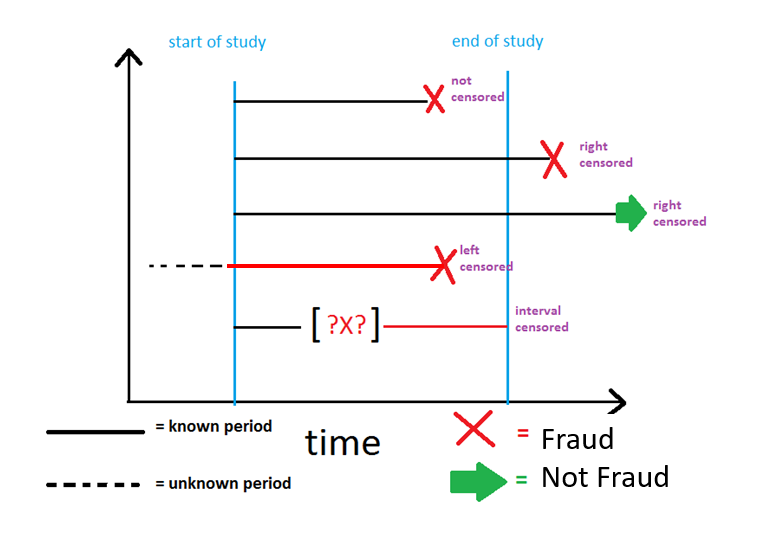
\includegraphics[width=12cm, height=6cm, scale=0.4]{images/01.png}

	
\end{frame}

\begin{frame}{Existing Methods}
	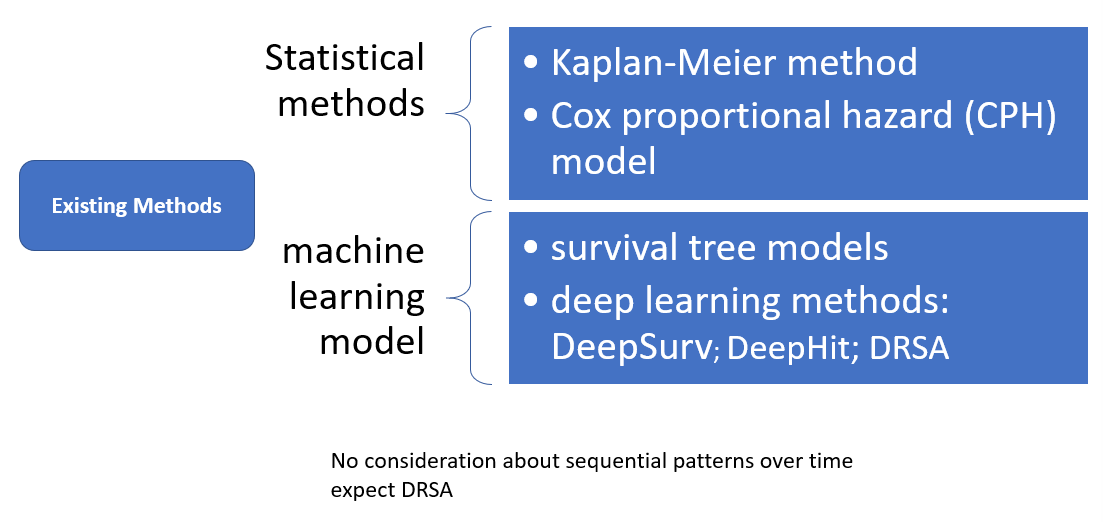
\includegraphics[width=11cm, height=6cm, scale=0.4]{images/02.png}

	
\end{frame}

\begin{frame}{Deep Recurrent Survival Analysis (DRSA)[6]}

	\begin{block}{Pros}
		\begin{itemize}
			\item No assumption about distributional forms
			\item Captures sequential patterns in the feature-time space
			\item First work ever, utilizes auto-regressive model for SA
			\item Handling censorship with unbiased learning
			\item Significant improvement against both stat. methods and ML methods
		\end{itemize}
		
	\end{block}
	
\end{frame}

\begin{frame}{Model diagram}
	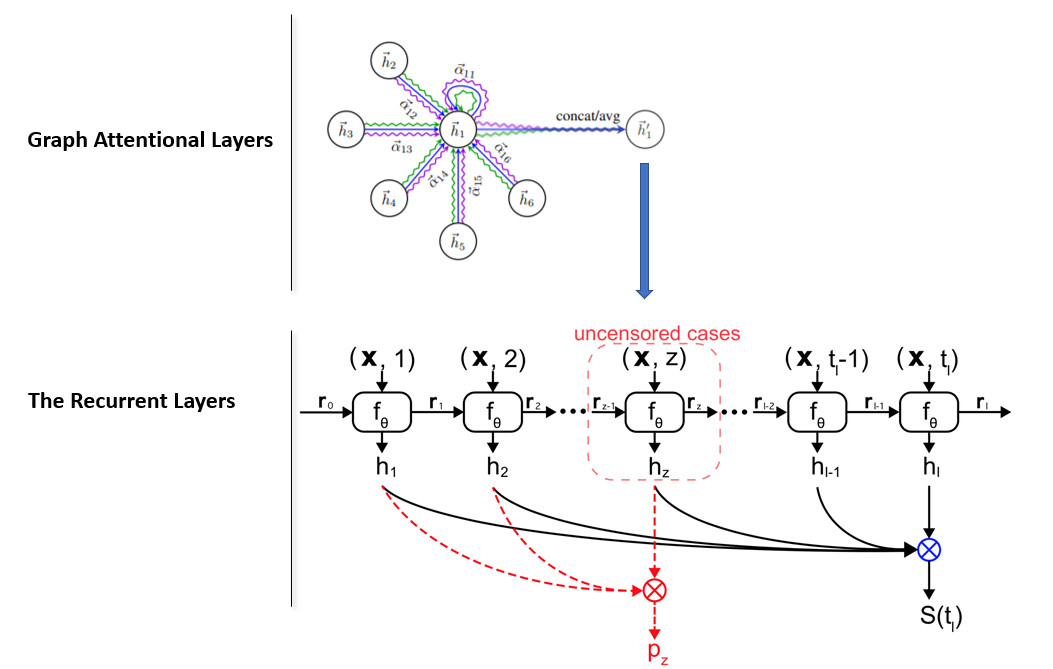
\includegraphics[width=12cm, height=6cm, scale=0.4]{images/03.png}

	
\end{frame}

% \section{References} \subsection{}

% \begin{frame}[allowframebreaks]{References}
	
% 	\printbibliography[heading=none]
	
% \end{frame}




% \end{document}

